\section{Results}
\label{sec:results}
In this section we start with an overview  of our feature enhancements. Then, we follow with a discussion of the bugs we identified in tiptop.

\subsection{Feature Enhancements}
Roughly, we enhanced tiptop with two new features.
First, we enhanced the default screen to include the number of threads per process.
Then, we added into tiptop the the cross-platform Performance Application Programming Interface (PAPI)~\cite{Mucci99papi:a} library, this enables a new, and more robust way, for tiptop to access performance counters.
We will discuss each of these feature in turn.

\subsubsection{Thread count on main screen}
The primary focus for tiptop is to enable a user to view hardware counters in real-time.
However, there are other variables that can indirectly influence hardware performance.
As an example, say a developer wants to investigate the effect of inter-thread cache contention on the performance of their application.
Especially in cases when the number of threads in a process is not deterministic, it would be valuable to have the thread count on the tiptop screen.
Therefore, we enabled tiptop to display the number of threads per process, and we included this feature on the default screen.

In our implementation we added hooks to the XML configuration logic to enable the ability to display the number of threads per process.
This involved adding code at multiple layers, including a call that exposed thread count from tiptops's data-gathering layer to the layer that handles presentation logic.
In addition, tiptop has multiple modes, which influence the filter that is applied to the processes/threads to be displayed.
As an example, tiptop can be run with the \texttt{-H} flag, in order to show per-thread information, rather than per-process.
In such a case we do not want to display thread count, and our implementation includes logic such that thread count only appears in the case when we filter by processes.

In the testing of this feature we did the following, using Python and C.
\begin{enumerate}
\item Execute a C program that spawns $N$ threads.
\item Start tiptop in batch mode.
\item Execute tiptop, parse the output and verify that tiptop displays $N$ threads for the long-running C process.
\end{enumerate}

Our tests passed on Ubuntu 12.04 executing a simple C program that invokes threads through the pthreads library, for values $N\in\{1,10,100\}$.
In Figure~\ref{fig:tiptop-threads} we have a screenshot of the enhanced default screen with the thread-count column, \texttt{\#TH}, highlighted.

\begin{figure}[t]
\footnotesize
\centering
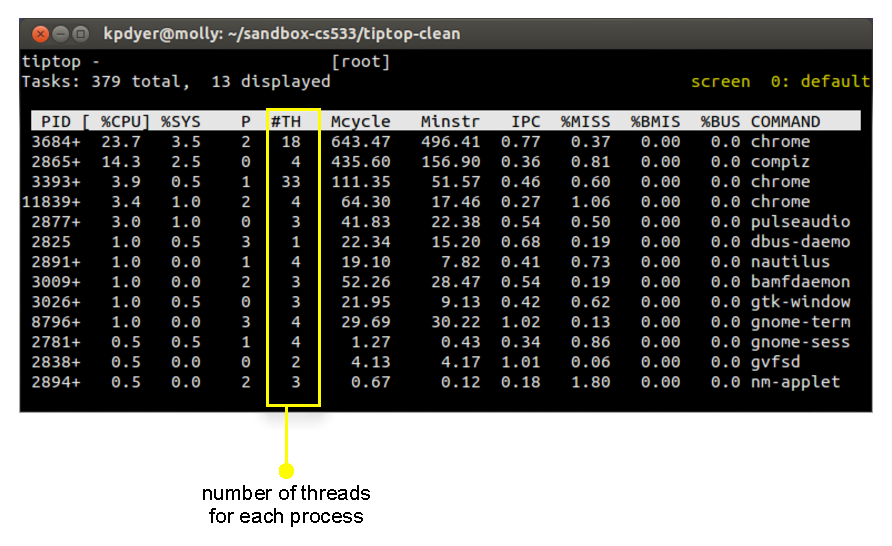
\includegraphics[width=.7\textwidth]{tiptop-threads}
%\hspace{.1in}
%\includegraphics[width=0.48\textwidth]{tiptop-default-screenshot-1}
\caption{A screenshot of the enhanced tiptop homescreen, showing the number of threads in each process.}
\label{fig:tiptop-threads}
\end{figure}

\subsubsection{Integration with the PAPI library}
\begin{figure}[t]
\footnotesize
\centering
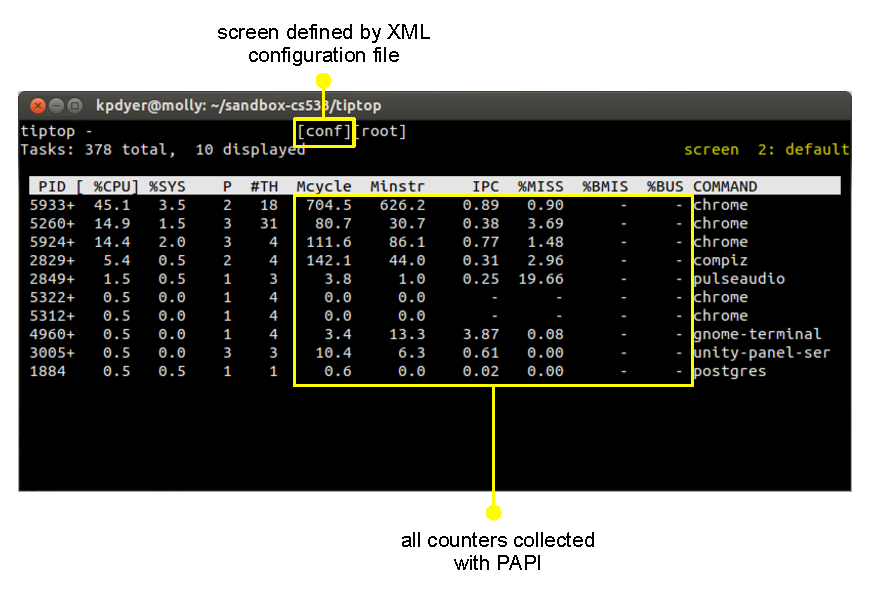
\includegraphics[width=.7\textwidth]{tiptop-papi}
%\hspace{.1in}
%\includegraphics[width=0.48\textwidth]{tiptop-default-screenshot-1}
\caption{The tiptop home screen implemented using the PAPI API. One side effect of using PAPI is that zero-values appear as \texttt{-} on the tiptop output. This was an inadvertent side-effect, but makes the screen more readable.}
\label{fig:tiptop-papi}
\end{figure}

As our next feature for tiptop, we integrated support for the Performance Application Programming Interface (PAPI) library.
The PAPI library is a cross-platform API for accessing hardware performance counters.
Roughly, it is a interface that removes the complexity involved in accessing hardware performance counters.

Consider the following concrete example for why integration with PAPI enhances tiptop.
The man page for tiptop gives the following example for a way to manually specify a counter that records the number of issued mico-ops on Sandy Bridge:
\begin{verbatim}
  <counter alias="uops_issued"
           config="0x010e"
           type="RAW"
           arch="x86"
           model="06_2A" />
\end{verbatim}
Then we must construct the column on the tiptop screen, too, which references the \texttt{uops\_issued} counter:
\begin{verbatim}
  <column header=" U Ops"
          format="%5.1f"
          expr="uops_issued" />
\end{verbatim}
The values for \texttt{config} and \texttt{model} in the \texttt{counter} tag are hardware-specific, and require that the user identifies the appropriate values in architecture-specific documentation in order to implement an alias, which can then be used to construct a column in a custom tiptop screen.
Indeed, it is less than ideal that a user must specify magic numbers for their CPU.
What is more, this is not portable, an alias for \texttt{uops\_issued} on a different platform will require different \texttt{config} and \texttt{model} values.
This is certainly a nightmare when developing a tiptop screen that may be used across multiple platforms.

Fortunately, PAPI makes life much easier.
Instead of having to specify a hardware-specific counter macro, then reference the macro for display, our new feature enables a user to specify the PAPI event directly.
There are 103 counter events specified in PAPI 5.0.1, and our integration with PAPI enables a user specify the PAPI-defined macro.
As an example, the following declaration would be able to integrate directly into the tiptop XML file
\begin{verbatim}
  <column header=" U Ops"
          format="%5.1f"
          expr="PAPI_FP_OPS" />
\end{verbatim}
It is then up to PAPI to determine the correct hooks for a hardware counter, and the burden is not on the user to identify magic numbers.
This is cross-platform, as far as PAPI supports the specific counter specified.
Hence, the user does not have to specify a custom hardware-specific \texttt{counter} macro, and a single XML file can be specified and deployed across multiple system.
In addition, this is backwards compatible with previous versions of tiptop configurations files, and the prefix \texttt{PAPI\_} for an \texttt{expr} attribute in a \texttt{column} tag, is a flag for tiptop to call PAPI, rather than using a direct kernel call for hardware counters.

In addition to a cleaner interface for accessing hardware counters, PAPI implements multiplexing for hardware counters, which enables a user to specify more counters that are permitted by the hardware.
As previously mentioned, if the underlying architecture is a Pentium III, tiptop is limited to two hardware counter events. However, PAPI implements multiplexing via high-precision timeslice sharing. This means that hardware counters are rotated, by default, every 100ms such that values can be obtained for all requested counters.
If we, say, specify four hardware events to monitor, in a 200ms window PAPI would monitor two hardware events for the first 100ms, then rotate to monitor the other two hardware events for the remaining 100ms.

Multiplexing does present limitations, if a user wanted to display a value such as instructions per second, this would require additional logic in order to know the amount of time that a specific counter was active.
We will leave this edge-case as future work.

As an additional feature, integration with PAPI enables tiptop to support a broader range of kernels. Currently, tiptop supports Linux kernels 2.6.31 and above.
PAPI supports Linux kernels 2.6.31 and above out of the box, and supports kernels 2.6.30 and below with a kernel patch.
Tiptop is not compatible with the PAPI patch for pre-2.6.31 kernels, and would require further modification to work for pre-2.6.31 kernels.
Hence, the PAPI integretation enables a greater range of kernel support without directly modifying tiptop.

\begin{figure}[t]
\footnotesize
\centering
\begin{tabular}{lrr}
\toprule
field & default expression & PAPI expression \\
\midrule
Millions of cycles (Mcycle) & \texttt{delta(CYCLE) / 1000000} & \texttt{PAPI\_TOT\_CYC / 1000000} \\
Millions of instructions (Minstr) & \texttt{delta(INSN) / 1000000} & \texttt{PAPI\_TOT\_INS / 1000000} \\
Instructions per Cycle (IPC) & \texttt{delta(INSN) / delta(CYCLE)} & \texttt{PAPI\_TOT\_INS / PAPI\_TOT\_CYC} \\
Instruction cache miss \% (\%MISS) & \texttt{100 * delta(MISS) / delta(INSN)} & \texttt{100 * PAPI\_L1\_ICM / PAPI\_TOT\_INS} \\
Branch misprediction \% (\%BMIS) & \texttt{100 * delta(BR) / delta(INSN)} & \texttt{100 * PAPI\_BR\_MSP / PAPI\_TOT\_INS} \\
\bottomrule
\end{tabular}
\caption{The expression changes required in the tiptop XML configuration file in order to use PAPI, instead of the default direct call to the Linux kernel. The previous expression still work, and the new PAPI macros simply extend the range of hardware counters that can be accessed from tiptop.}
\label{fig:tiptop-papi-expressions}
\end{figure}

\paragraph{Challenges in integrating PAPI with tiptop.}
When integrating PAPI with tiptop, we encountered a number of challenges.
First, PAPI's documentation was nearly non-existent when describing its ability to multiplex and monitor external processes.
A correct implementation required extensive reading and searching through the PAPI mailing lists.
In addition, understanding tiptop's workflow and the correct functions to call to release the hardware counters via PAPI took some effort, too.

\paragraph{Case Study: Building the tiptop default home screen with PAPI.}
In order to demonstrate the flexibility of our PAPI integration and its correctness, we implement the default tiptop screen using PAPI, instead of tiptop's default behavior of using direct kernel calls.
In Figure~\ref{fig:tiptop-papi} we have a screenshot of the tiptop homescreen, implemented by building an XML file that references PAPI macros.
We first notice that the top of the screen the \texttt{[conf]} flag, which indicates that the tiptop screen is specified by the an XML configuration file.

In Figure \ref{fig:tiptop-papi-expressions} we have a listing of the current tiptop expression used to build the default screen, and the alternative expression that can now be used to access counter via PAPI. These expressions can be mixed and matched within the same XML file.

As an example of another benefit of PAPI exposed by building the home screen, the tiptop interface exposes \texttt{MISS} (Figure \ref{fig:tiptop-papi-expressions}) as \texttt{PERF\_COUNT\_HW\_CACHE\_MISSES}, which in the Linux kernel references either L1 or L2 Instruction Cache misses\footnote{\texttt{\url{https://lkml.org/lkml/2010/11/1/131}}}.
Depending upon your kernel version, for \%MISS in Figure \ref{fig:tiptop-papi-expressions} with return either Level 1 or Level 2 instruction cache misses. However, it is clear from the PAPI macro that we are returning the Level 1 instruction cache miss. If we, say, wanted to report Level 2 instruction cache misses instead, we simply replace \texttt{PAPI\_L1\_ICM} with \texttt{PAPI\_L2\_ICM}.
Alternatively, if we wanted, instead, the Level 3 data cache miss, we could use the macro \texttt{PAPI\_L3\_DCM}.

\subsection{Bug Fixes}
In our initial attempt to understand tiptop and its range of features we encountered an anomaly.
In some cases a question mark would appear, instead of a value from the hardware performance counter.
This would happen consistently for programs such as the Chrome\footnote{\texttt{\url{http://www.google.come/chrome}}} web browser, and would happen sporadically for other applications.
In Figure~\ref{fig:tiptop-bug} we have a screenshot that highlights this bug.
Upon investigation, we identified two separate issues that lead to this error condition.
\begin{figure}[t]
\footnotesize
\centering
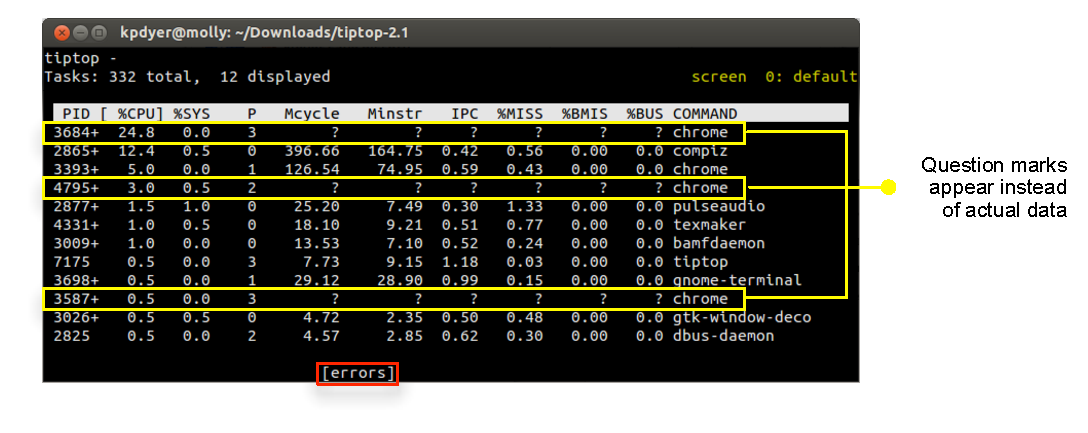
\includegraphics[width=.9\textwidth]{tiptop-bug}
%\hspace{.1in}
%\includegraphics[width=0.48\textwidth]{tiptop-default-screenshot-1}
\caption{A screenshot of the manifestation of the two bugs identified in our development. When tiptop is unable to determine the values associated with a process it ouputs a question mark instead. As we can see, tiptop failed to gather statistics for three of the four Chrome processes in the above screenshot, at the bottom of the screen, in the red box, tiptop reports that \texttt{[errors]} occurred.}
\label{fig:tiptop-bug}
\end{figure}

\paragraph{Bug 1: Too many open file descriptors.}
First, a bit of background. Linux systems include a \texttt{limits.conf} file which enables a systems administrator to have fine-grained control over the system resources used by users and groups.
As an example, it is possible to specify the maximum priority of a process run by a specific user or group, or even the maximum number of processes spawned by a specific user or group. Each resource has a \emph{hard} and \emph{soft} limit. Hard limits are enforced by the kernel and can only be modified by superusers. Soft limits are default values and can be manually raised per-user, up to the hard limit.
For example, Ubuntu 12.04 has a soft limit of 1024 open file descriptors per user, and a hard limit of 4096.
This means that a regular user can open up to 1024 file descriptors under normal circumstances, or can open up to 4096 file descriptors by explicitly requesting (to the kernel) for the soft limit to be increased to 4096.

In order to read hardware counters, tiptop opens five counters per process in its default configuration.
For each combination of process and hardware counter, a file descriptor is opened.
As we can can see in the screenshot for Figure~\ref{fig:tiptop-bug}, my desktop had 332 running processes.
Hence, we now have a problem.
We have 332 processes, five hardware counters per process, so we have exceeded our soft limit for the number of file handlers open by requesting to open $332\cdot 5 = 1660$ file descriptors.

As a stopgap solution to this problem, we explicitly request for our soft file descriptor limit to be increased to the hard limit. This may be performed by fetching the hard limit from \texttt{/proc/N/limits}, then making a call to the \texttt{setrlimit} function, which is provided by \texttt{sys/resource.h}.
Unfortunately, increasing the open file descriptor limit beyond the hard limit requires superuser permission.
Our solution, raising the soft limit to the hard limit, is consistent with other open source project that have encountered this issue, such as Wine\footnote{\texttt{\url{https://bugs.launchpad.net/ubuntu/+source/linux/+bug/663090}}}.
A more robust solution for this bug is an open problem and would require fundamental changes to the design of tiptop, we talk about possible solutions in section~\ref{sec:conclusion}.

The testing for this was not straightforward due to a different bug, which we will discuss next.
In order to verify our fix for this bug we ran tiptop as root, with root having a hard number of file descriptor set to 4096 and soft set to 1024. (By default, root has a soft limit of 4096 and hard limit of 8192 on Ubuntu 12.04.)
We may then run the version of tiptop that uses the soft limit and we get the following output.
\begin{verbatim}
19884+   4.6   0.0    0        ?        ?     ?      ?      ?     ? chrome
...
19818+   0.5   0.5    0        ?        ?     ?      ?      ?     ? firefox
\end{verbatim}

Simultaneously, we run the enhanced version of tiptop that explicitly requests a file descriptor limit to be raised to the hard limit, and we get the following output.
\begin{verbatim}
19884+   4.3   0.0    0 19327.35 19327.35  1.00   0.00   0.00   0.0 chrome
...
19818+   0.5   0.5    0  8589.93  8589.93  1.00   0.00   0.00   0.0 firefox
\end{verbatim}

We verify by that this bug is solved by checking that no value in the tiptop output has a question mark. A more robust testing strategy will require an enhanced error reporting layer for tiptop, which distinguishes between different types of hardware counter read failures. However, an enhanced error reporting layer is beyond the scope of this project.

\paragraph{Bug 2: \texttt{EACCES}, permission denied.}
A second cause of ``questions marks" in the tiptop output has been traced to an \texttt{EACCES} permission denied error returned by the kernel, and is isolated to only a few applications, such as Chrome and the gnome-keyring-daemon, to name a few.
This condition only occurs when running tiptop as a regular user.
We contacted the lead developer of tiptop, Erven Rohou, in order to determine the cause of this problem.
This was an unknown bug, but it can be avoided by running tiptop as root.
Unfortunately, we have no further progress towards a solution to this bug.